\makeatletter
\def\input@path{{../../}}
\makeatother
\documentclass[../../main.tex]{subfiles}

\graphicspath{
	{../../img/}
	{../img/}
	{img/}
}

\begin{document}
	
\begin{rems}

\;

\begin{enumerate}
	\item В обосновании достаточности доказанной теоремы существенную роль 
	играло предположение о непрерывности дифференцируемой функции 
	$ u = \Re f(z) $ и $ v = \Im f(z) $. В общем случае  можно отказаться 
	от него, но при условии этом доказательство значительно усложнится.
	\item Используя условие Коши-Римана \eqref{lec28:17} из \eqref{lec28:21} 
	также имеем:
	\begin{equation}
	\label{lec29:22} 
	f'(z) = v_y' - iu_y' = \left[u_y' = v_x'\right] =
	v_y' - iu_x' = \left[v_y' = u_x'\right] = u_x' + iv_x' = u_x' - iu_y'
	\end{equation}
	\item $ \forall c, y \in \R $ рассмотрим 
	$ \left[\begin{gathered}
		F(x, y) = f(x + iy) =\\
		=u + iv, u, v \in \R
	\end{gathered}\right] $ 
	и, применяя дифференцирование сложных ФКП получаем, что 
	\[ 
	F_x' = (f(z))_x' = f'(z)z_x' = \left[
	\begin{gathered}
		z = x + iy\\
		z_x' = 1
	\end{gathered}
	\right] = f'(z) = (u + iv)_x' = u_x' + iv_x'
	\]
	Аналогично
	\[ 
	F_y' = (f(z))_y' = f'(z)z_y' = \left[
	\begin{gathered}
	z = x + iy\\
	z_y' = i
	\end{gathered}
	\right] = if'(z) = \dots
	\]
	(Я так и не понял, что и в каком порядке у Никиты в конспекте идёт на \dots)
	Указанные действия поясняют смысл условий Коши-Римана \eqref{lec28:17}.
\end{enumerate}
\end{rems}
\begin{exmps}
\begin{enumerate}
	\item $ f(x) = z = x + iy, x, y \in \R $
	\[
	\begin{cases}
		u = \Re f(z) = x\\
		v = \Im f(z) = y
	\end{cases}
	\]
	Имеем 
	\[
	\begin{cases}
		u_x' = 1 = v_y'\\
		u_y' = 0 = -v_x'
	\end{cases}
	\]
	Условия \eqref{lec29:17} выполняются, значит ФКП является дифференцируемой,
	причём $ f'(z) = (z)' = \stackrel{\eqref{lec28:21}}{=} u_x' + iv_y' = 
	1 + i0 = 1 $, что согласуется с действительным случаем.
	\item $ f(z) = \overline{z} = x - iy, x, y \in \R $\\
	$ u = x, v = -y, \implies u_x' = 1 \neq -1 = v_y' \leftarrow $ 
	\eqref{lec29:17}. Условие Коши-Римана не выполняется $ \implies $ ФКП 
	не дифференцируема ни в одной точке.
	\item $ f(z) = z \Re z = x(x + iy) $
	\[
	\begin{cases}
		u = \Re f(z) = x^2\\
		v = \Im f(z) = xy
	\end{cases}
	\]
	\eqref{lec29:17}:
	\[
	\begin{cases}
		u_x' = 2x = x = v_y'\\
		u_y' = 0 = -y = -v_x'
	\end{cases} \implies
	\begin{cases}
		x = 0\\
		y = 0
	\end{cases}
	\]
	Значит рассматриваемая функция дифференцируема в точке $ z_0 = (0, 0) $.
	Причём
	$ f'(0) = u_x'(0, 0) + iv_x'(0, 0) = 0 $.
	\item $ f(z) = e^z = e^{x + iy} = e^x(\cos y + i\sin y), x, y \in \R $\\
	\[
	\begin{cases}
		u = \Re f(z) = e^x \cos y\\
		b = \Im f(z) = e^x \sin y
	\end{cases}
	\]
	Составим \eqref{lec29:17}:
	\[
	u_x' = e^x \cos y = e^x \cos y = v_y'\\
	u_y' = -e^x \sin y = -e^x \sin y = -v_x'
	\]
	Условие \eqref{lec29:17} выполнено $ \forall z \in \C $, 
	поэтому комплексная экспонента не является дифференцируемой функцией в $ \C 
	$, причём
	\[
	f'(z) = (e^z)' = u_x' + iv_x' = e^x \cos y + ie^x \sin y =
	e^x(\cos y + i\sin y) = e^{x + iy} = e^z
	\]
	что также согласуется с производной действительной экспоненты.
\end{enumerate}
\end{exmps}

Аналогичным образом находятся производные основных элементарных ФКП, 
и при этом, получаемые формулы будут естественным образом обобщаться для
соответствующих элементарных действительных функций. Например:
\[
\begin{gathered}
(\sin z)' = \cos z, (\cos z)' = -\sin z\\
(\tg z)' = \dfrac{1}{\cos^2 z}\\ 
(\ctg z)' = \dfrac{-1}{\sin^2 z}\\
(\Ln z)' = \dfrac{1}{z}\\
(\Arcsin z)' = \dfrac{1}{\sqrt{1 - z^2}}\\
(\Arccos z)' = \dfrac{-1}{\sqrt{1 - z^2}}\\
(\Arctg z)' = \dfrac{1}{1 + z^2}\\
(\Arcctg z)' = \dfrac{-1}{1 + z^2}
\end{gathered}
\]
\begin{exc}
	Записать соответствующие формулы для гиперболических 
	и обратных к ним функций.
\end{exc}

\section{Гармонические функции}

Как будет получено позжже из того, что ФКП $ f(z) $ дифференцируема в области
$ D \subset \C $, т.~е. $ \forall z \in D \implies f'(z) \in \C $, то она 
будет
в отличие от вещественных функций бесконечное число раз дифференцируема в $ D 
$.
Поэтому действительные функции 
\[
\begin{cases}
	u = u(x, y) = \Re f(z)\\
	v = v(x, y) = \Im f(z)
\end{cases}
\]
будут также бесконечное число раз дифференцируемы. Отсюда, используя условие
Коши-Римана \eqref{lec29:17} следует:
\[
\begin{gathered}
\exists u_{x^2}'' = (u_x')_x' 
\stackrel{\eqref{lec28:17}}{=}
[u_x' = v_y'] = (v_y')_x' = v_{yx}''\\
\exists u_{y^2}'' = (u_y')_y' 
\stackrel{\eqref{lec28:17}}{=}
[u_y' = -v_x'] = (-v_x')_y' = -v_{yx}''\\
\end{gathered}
\]
Из теоремы о равенстве смешанных производных ФКП следует, что 
$ u_{xy}'' = v_{xy}'' $. Поэтому $ u_{x^2}'' + u_{y^2}'' = v_{xy}'' - v_{xy}'' 
= 0 $.

Аналогично показывается, что $ v_{x^2}'' + v_{y^2}'' = \dots = 0 $.

(Кр. дифф ур-ие с частными производными используют дифференциальный оператор 
Лапласа)???:
\[
\D = \dfrac{d^2 (.)}{d x^2} + \dfrac{d^2(.)}{d y^2}
\]
Для дважды дифференцируемой $ F = F(x, y) $ имеем\[
\D F = \dfrac{d^2 F}{d x^2} + \dfrac{d^2 F}{d y^2} = 
F_{x^2}'' + F_{y^2}''
\]
В общем случак, если дважды дифференцируемая Ф2П $ F(x, y) $
удовлетворяет $ \D F = 0 $, то эта Ф2П называется гармонической функцией.
Из предыдущего следует, что действительная и мнимая части 
дифференцируемой ФКП являются гармоничесими функциями, т.~к.
$ \D u = 0, \D v = 0 $.

Если производная пара $ u = u(x, y), v = v(x, y) $ являются гармоническими 
функциями, 
удовлетворяющими условию Коши-Римана \eqref{lec28:17},
то она называется сопряжённой парой гармонических функций.

Можно показать, что любую дифференцируюмую ФКП можно с точностью до константы 
восстановить, зная лишь её действительную или мнимую часть.
\begin{exmp}
Найдём дифференцируюмую ФКП $ f(z) = u + iv, u, v\in \R $,
если $ u = \Re f(z) = 2xy $ и $ f(1 + i) = 2 $.\\
Проверим корректность постановки:
\begin{enumerate}
	\item[а)] $ u $~--- гармоническая функция.
	\[\D u = u_{x^2}'' + u_{y^2}'' = (2y)_x' + (2x)_y' = 0 \]
	\item[б)] \[
	\begin{cases}
		z_0 = 1 + i = x_0 + iy_0\\
		x_0 = 1, y_0 = 1
	\end{cases}
	f(1 + i) = u(x_0, y_0) + iv(x_0, y_0) = \left[
	\begin{gathered}
		u(1, 1) = 2\\
		v(1, 1) = 0
	\end{gathered}
	\right] = 2
	\]
	Для восстановления надо найти $ v(x, y) $.\\
	$ v(1, 1) = 0 $, т.~к. $ u, v $~--- комплексно-сопряжённая пара
	гармонических функций, то в силу \eqref{lec28:17}
	\[
	\begin{cases}
		v_x' = -u_y' = -2x\\
		v_y' = u_x' = 2y
	\end{cases}
	\]
	Используя непрерывность интеграла \[ 
	v = -2\int x dx = -x^2 + C(y) 
	\implies v_y' = C'(y) = 2y \implies 
	C(y) = 2\int y dy = y^2 + C \implies \]\[ \implies
	v(x, y) = -x^2 + y^2 + C
	\]
	Используя $ v(1, 1) = 0 \implies 1 - 1 + C = 0 \implies C = 0 \implies 
	v(x, y) = y^2 - x^2
	$. Значит, $ f(z) = u + iv = 2xy + i(y^2 - x^2) =
	-i(2ixy - y^2 + x^2) = -i(x + iy)^2 = -iz^2
	$
\end{enumerate}
\end{exmp}

\section{Геометрический смысл модуля и производной аналитической ФКП}

Далее дифференцируемую в каждой точке $ D $ ФКП $ f(z) $
будем называть аналитической в $ D $.

Пусть $ f(z) $ аналитическая в некоторой окрестности $ z_0 \in D $ и 
$ f'(z_0) \neq 0 $. Тогда
\[
f'(z_0) = k e^{i\phi},
\begin{cases}
	k = \abs{f'(z_0)} > 0\\
	\phi = \arg f'(z_0) \in ]-\pi; \pi]
\end{cases}
\]
Придадим $ z_0 \in D $ достаточное малое произвольное приращение 
$ \D z \in \C $ так, чтобы $ z_0 + \D z $ (???не понимаю слова???) в 
окрестности
дифференцируемой $ f(z) $. Тогда для
\[
w = f(z) \implies \exists \lim\limits_{\D z \to 0} 
\dfrac{\D w(z_0)}{\D z} = f'(z_0)
\]
Отсюда для достаточно малых приращений получаем
\[
\abs{\dfrac{\D w(z_0)}{\D z}} \approx \abs{f'(z_0)} = k > 0
\implies \abs{\D w(z_0)} \approx k\abs{\D z}
\]
Для $ \phi \arg f'(z_0) $ получаем $ \phi \approx \arg 
\dfrac{\D w(z_0)}{\D z} = \arg \D w(z_0)  $~---$ \arg \D z \implies
\alpha = \arg \D w(z_0) \approx \phi + \arg \D z
$
\begin{equation}
\label{lec29:23}
\begin{cases}
	\abs{\D w (z_0)} \approx k\abs{\D z}\\
	\arg \D w(z_0) \approx \phi + \arg \D z
\end{cases}
\end{equation}
имеет следующий геометрический смысл:\\
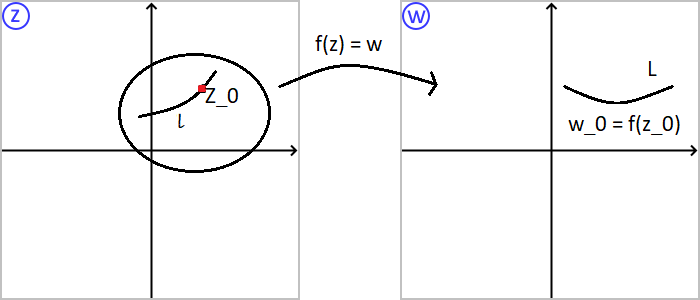
\includegraphics{lec29_1}\\
Первое из равенств \eqref{lec29:23} с учётом того, что модуль комплексного 
числа
есть длина радиус вектора этой точки, говорит о том, что в достаточно 
малых окрестностях точки $ z_0 $ длины образа $ L $ и прообраза $ l $ связаны 
соотношением:
длина $ L \approx k * $ длина $ l $. 
Поэтому если $ k = \abs{f'(z_0)} > 1 $, то имеем растяжение длин, 
а если $ 0 < k < 1 $~--- сжатие.
Далее, изображая $ l $ и $ L $ на совмещённом чертеже, где 
$ z_0 $ и $ w_0 $ совпадают для касательных в совсмещённой точке к этим 
линиям, имеем:\\
\begin{center}
	$
	\begin{gathered}
	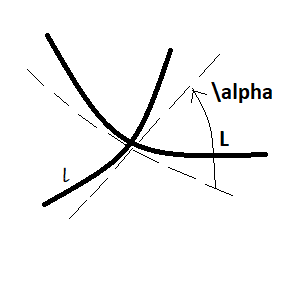
\includegraphics{lec29_2}\\
	\alpha \approx \arg \D w(z_0) \approx \phi + \arg \D z
	($поворот на $ \alpha )
	\end{gathered}
	$
\end{center}
Это является геометрическим смыслом аргумента $ ???A??? $.

Далее отобрав $ f(z) = w $(необязательно дифференцируюмую),
к каждой точке $ z_0 \in D $ сохраняя построение ???не понял слово??? 
и поворот, будем называть ???конформными???.

Если при этом ориентация образа сохраняется, то такое конформное отображение
называется отображением $ I $ рода, иначе $ II $ рода.

Можно показать, что если $ w = f(z) $ конформное отображение $ I $ рода, 
то $ w = \overline{f}(z) $~--- будет конформным отображением $ II $ рода.

Используя геометрический смысл модуля производной аналитической ФКП
можно показать, что если в $ D \subset \C $ имеется гладкая линия
$ l \subset D $, заданная $ z = x(t) + iy(t),\ t_1 \leq t \leq t_2 $, то тогда
для $ L = f(l) $ образа $ l $ при отображении $ w = f(z) $ является 
аналитической функцией, имеем:\\
Длина $ L = \int\limits_{l} \abs{f'(z(t))} dt = 
\int\limits_{l} \sqrt{(x'(t))^2 + (y'(t))^2} dt $.
Аналогично, если рассматриваемая квадратная область $ G \subset D $, 
то для площади $ G $: S = площадь $ f(G) $ образа $ G $ при ???анал??? 
отображении $ w = f(z) $ имеем:
\[
S = \iint_{G} \abs{f'(z)}^2 dx dy
\]


\end{document}
